%section-start setup
\documentclass{beamer}
%section-start declare document information!
\title[Short Example Title]{Example Title}
\subtitle{TODO Example Subtitle}
\author{Hannah Nelson}
\institute{University of California, Santa Barbara}
\date{2026}
%section-end
%section-start load packages!
\usepackage{graphicx}
\usepackage[backend=biber]{biblatex}
\usepackage{xcolor}
\usepackage{soul} % use the package named soul by Melchior Franz for highlighting
%section-end
%section-start add bibliography
\addbibresource{refs.bib}
%section-end
%section-start define macros
%section-start shiftleft
% A simple command to shift stuff left. meant to shift itemizes left because beamer doesn't play well with left margins for some reason.
\newcommand\shiftleft[1]{
    \begin{columns}
        \begin{column}{0.1\textwidth}
        \end{column}
        \begin{column}{0.9\textwidth}
            #1
        \end{column}
    \end{columns}
}
%section-end
%section-end
%section-end
%section-start document
\begin{document}
%section-start titlepage
\begin{frame}
\titlepage
\end{frame}
%section-end
%section-start Example Image Slide
\begin{frame}
    \frametitle{Example Image Slide}
    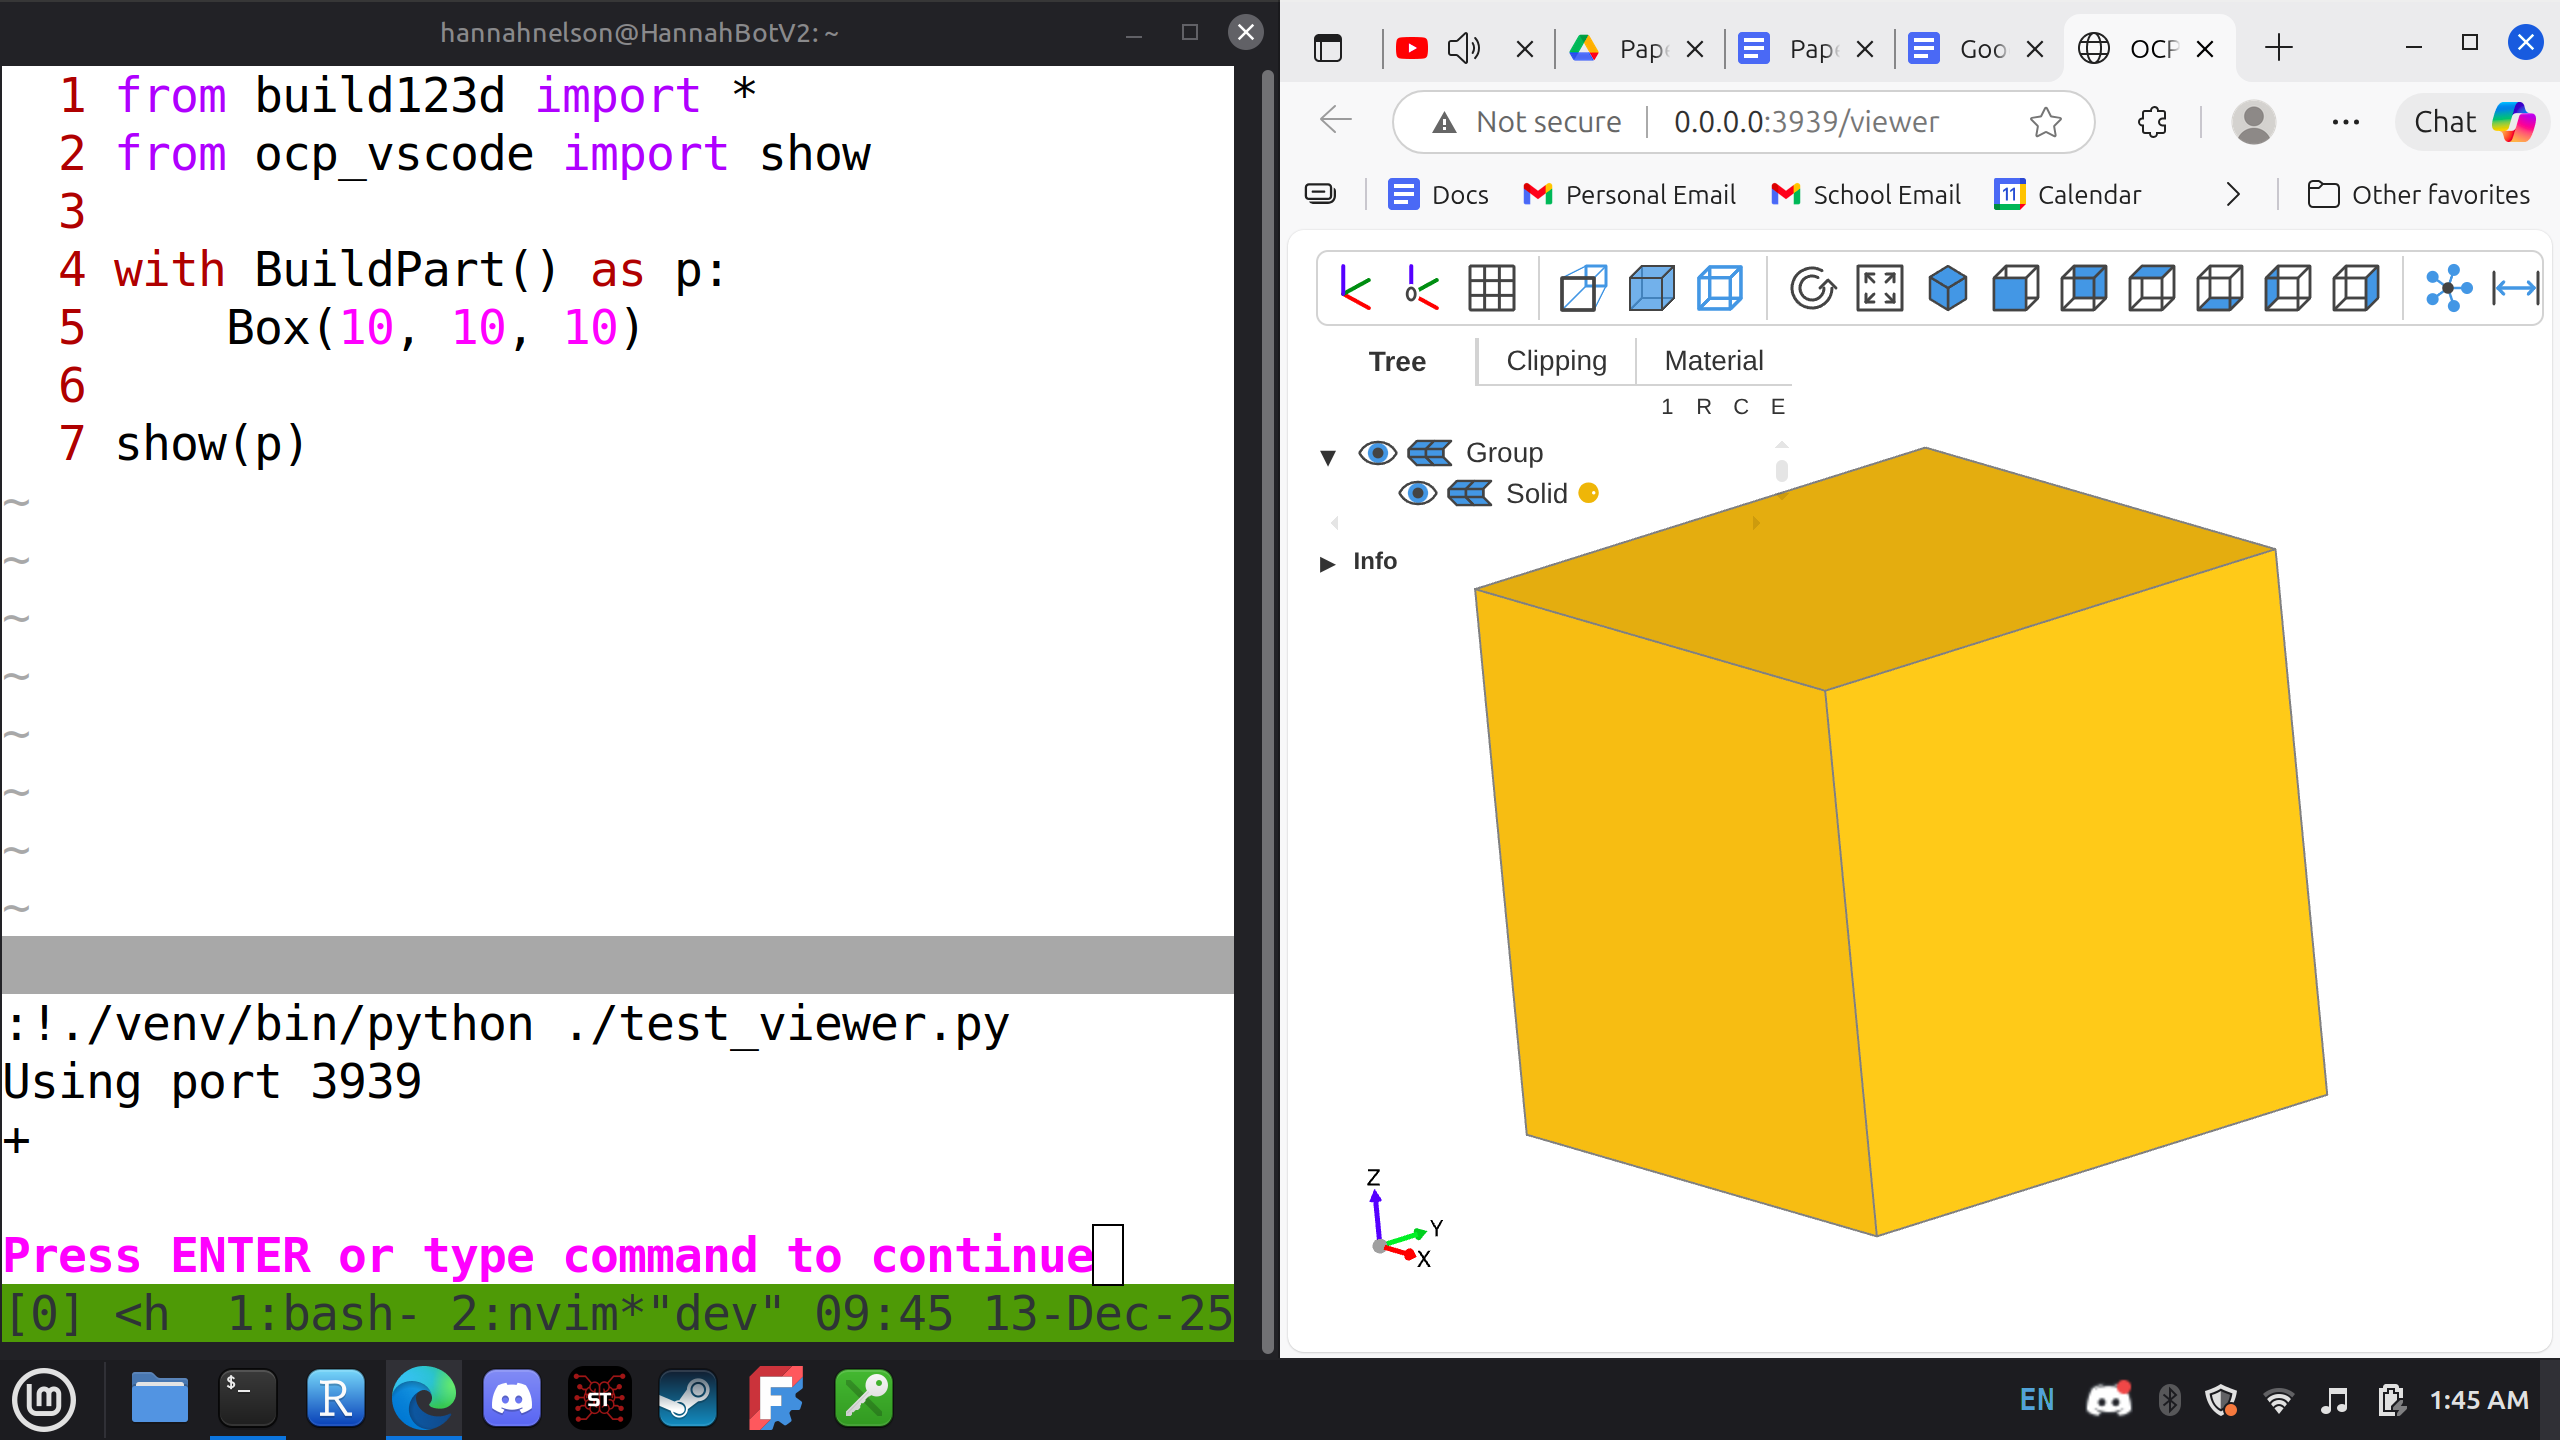
\includegraphics[totalheight=6cm]{resources/example_image.png}
\end{frame}
%section-end
%section-start Example Slide
\begin{frame}
    \frametitle{Example Slide}
    \shiftleft{
        \begin{itemize}
            \item[The Paper:]
                \citetitle{TODO_remove_this_demo_cititation}
            \item[The Problem:]
                Random Text stochastic without forin what is the maxima of the defined boundary which into the vibe.
            \item[The Difficulty:]Words Text things to say.
        \end{itemize}
    }
\end{frame}
%section-end
%section-start Citations
\begin{frame}
\frametitle{Citations}
    \printbibliography
\end{frame}
%section-end
\end{document}
%section-end
